\documentclass{article}
\usepackage[margin=0.7in]{geometry}
\usepackage{graphicx}
\usepackage{color}
\usepackage{hyperref}
\graphicspath{ {/asay/Desktop/images/} }
\usepackage{xepersian}




\title{پاسخ تمرین شماره ۵ درس معماری کامپیوتر }


\author{امیر حسین عاصم یوسفی \\ ۹۶۱۱۰۳۲۳}
\settextfont{B Nazanin}

\begin{document}
	\maketitle
	
\section*{سوال ۱}
با توجه به این طولانی ترین تاخیر مربوط به 
\lr{Mem}
می باشد که برابر با ۲ نانوثانیه می باشد و این که تاخیر رجیستر های میانی ۰/۱ نانوثانیه هستند پس برای 
\lr{Clock Time}
جدید داریم  : 
\begin{center}
	\lr{Clock Time new = 2ns + 0.1ns = 2.1ns}
\end{center}
برای این که تاثیر
\lr{stall}
را در نظر بگیریم باید 
\lr{CPI}
را برای زمانی که 
\lr{stall}
داریم طبق فرمول زیر به دست آوریم : 
\begin{center}
	\lr{CPI = IdealCPI + stall cycles}
\end{center}
در این جا 
\lr{IdealCPI = 1}
در نظر می گیریم و چون به ازای هر ۴ دستور یک 
\lr{stall}
داریم پس 
\begin{center}
	\lr{stall cycles  = 1/4 = 0.25ns}
\end{center}
بنابراین طبق فرمول گفته شده 
\textcolor{red}{\lr{new CPI (with Stall)  = 1 + 0.25 = 1.25ns}}\\
تا به حال مقادیر 
\lr{CT}
و 
\lr{CPI}
را برای معماری 
\lr{Pipeline}
به دست آوردیم حال  
\lr{Speedup}
راطبق فرمول زیر به دست می آوریم  : 
\begin{center}
 \lr{SpeedUp = $ \frac{Single  \  cycle \  EXE  \ time}{Pipeline \  EXE  \ time }$}\\
 \lr{Execution TIme  = CPI . IC  . Cycle time}
\end{center}
حال با توجه به بالا داریم  : 
\begin{center}
	\lr{SpeedUp = $\frac{IC \times 1 \times 7}{IC \times 1.25 \times 2.1} = \frac{7}{2.625}$ = 2.67 ns}
\end{center}
\hrule
\section*{سوال ۲}
برای این سوال با توجه به قانون 
\lr{Amdahl}
داریم  : 
\begin{center}
	\lr{SpeedUp = $\frac{1}{\frac{P}{N} + S}$}
\end{center}
که در این جا 
\lr{P}
نشان دهنده بخشی است که به صورت 
\lr{Parallel}
نوشته شده و 
\lr{N}
نشان دهنده تعداد پردازنده ها و 
\lr{S}
بیانگر بخشی است که به صورت موازی نوشته نشده است . پس داریم  : 
\begin{center}
	\lr{SpeedUp = $\frac{1}{\frac{x}{4}+(1-x)} = 2 \rightarrow x = \frac{2}{3}$ $\Rightarrow$ x = 66\%}
\end{center}
بنابراین باید ۶۶ درصد از برنامه را به صورت موازی نوشت تا اجرای برنامه بر روی این ۴ پردازنده ۲ برابر سریع تر شود  . 
\hrule
\section*{سوال ۳ }
با استفاده کردن از حافظه نانو که در 
\lr{Nano Programming}
مورد استفاده قرار می گیرد که از یک 
\lr{Control Storage Organization}
دو سطحی استفاده میکند که سطح بالاتر
\lr{Micromemory}
 از نوع عمودی یا 
\lr{(Vertical)}
می باشد که آدرس مورد نیاز سطح پایین تر خود یا همان 
\lr{Nano Memory}
را تامین می کند . \\
این سطح وظیفه تولید کردن سیگنال های کنترلی رادارند و ویژگی آن ها صرفه جویی در حجم ریز برنامه واحد کنترل می باشد  . \\
بدون وجود این نوع حافظه اگر بخواهیم به صورت یک سطحی 
\lr{Single Layer}
جلو برویم حجم ریز برنامه به صورت زیر است :‌ 
\begin{center}
	\lr{\# of control memory bits = \# of control signals * \# of microinstructions = 50 * 180 = 9000 bit}
\end{center}
ولی اگر با حافظه های نانو جلو برویم با توجه به این که  از یک چارت عملیاتی با ۱۱۴ نقطه کنترلی  استفاده می کنیم داریم  : 
\begin{center}
	\lr{First layer (Microstore) = 180 * 8  = 1440 bit}
	\\
	\lr{Second layer (NanoMemory) = 114 * 50  = 5700 bit }
\end{center}
بنابراین در صورت استفاده از حافظه نانو حداقل 
\textcolor{red}{\lr{9000 - (5700+1440) =1860 bit}  }
در حجم ریز برنامه صرفه جویی می شود  . 
\hrule
\section*{سوال ۴}
\hrule
\section*{سوال ۵ }
با توجه به این که 
\lr{Full Forwarding}
داریم بنابراین مراحل به شکل زیر می باشد   : 
\begin{center}
	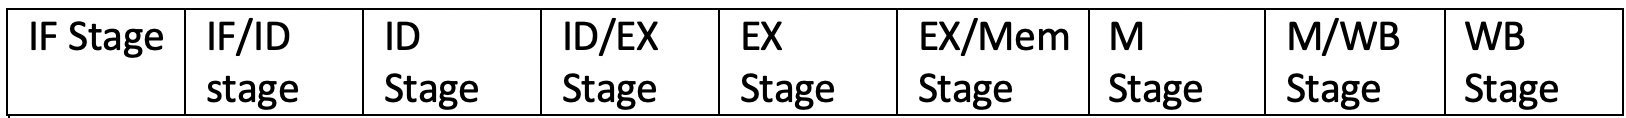
\includegraphics[width=1\textwidth]{q5p1}
\end{center}
با توجه به این مراحل و ترتیب دستورات ذکر شده در صورت سوال می توان فهمید که 
\lr{\$6}
که در عملیات تفریق جزو عملوند ها می باشد در مرحله 
\textcolor{red}{\lr{M/WB}}

تولید می شود  و عملوند دوم این عملیات یعنی 
\lr{\$8}
در مرحله 
\textcolor{red}{\lr{EX/M}}
تولید می شود  . 
\section*{سوال ۶}
برنامه به صورت زیر می باشد ‌‌:
\begin{center}
	\begin{enumerate}
		\item \lr{sub \$a3,\$a2\$a1}
		\item \lr{and \$v1,\$a3,\$v4}
		\item \lr{or \$v2,\$v5,\$a3 }
		\item \lr{lw \$v4,100(\$a3)}
		\item  \lr{sw \$v2,100(\$a3)}
	\end{enumerate}
\end{center}
\subsection*{\textcolor{red}{الف}}
با توجه به شماره گذاری های بالا به مخاطرات زیر می رسیم  : 
\subsubsection*{1}
بین خطوط 
\textcolor{red}{2}
و 
\textcolor{red}{۱}
که بر سر رجیستر 
\lr{\$a3}
با یک دیگر 
\textcolor{blue}{\lr{Data Hazard}}
دارند . 
\subsubsection*{2}
بین خطوط
\textcolor{red}{۴}
و 
\textcolor{red}{۱}
بر سر رجیستر 
\lr{\$a3}
با یک دیگر 
\textcolor{blue}{\lr{Data Hazard}}
دارند . 
\subsubsection*{3}
بین خطوط 
\textcolor{red}{5}
و 
\textcolor{red}{۳}
بر سر 
\lr{\$v2}
با یک دیگر 
\textcolor{blue}{\lr{Structure Hazard}}
دارند  . 
\subsubsection*{4}
خطوط 
\textcolor{red}{5}
و
\textcolor{red}{۱}
بر سر 
\lr{\$a3}
با یک دیگر 
\textcolor{blue}{\lr{Data Hazard}}
دارند  . 
\subsubsection*{5}
بین خطوط 
\textcolor{red}{۳}
و
\textcolor{red}{۱}
بر سر 
\lr{\$a3}
با یک دیگر 
\textcolor{blue}{\lr{Data Hazard}}
دارند . 
\subsubsection*{6}
بین خطوط 
\textcolor{red}{5}
و
\textcolor{red}{۴}
بر سر 
\lr{\$a3}
با یک دیگر 
\textcolor{blue}{\lr{Structure Hazard}}
دارند . 
\subsection*{\textcolor{red}{ب}}
با توجه به قسمت قبل پردازنده برای دستور دوم باید 
\textcolor{red}{2}
کلاک متوقف شود بنابراین برای این که دستورات به درستی اجرا شوند در کل ۲ 
\lr{Stall}
داریم که به صورت زیر می باشد  : 
\begin{center}
	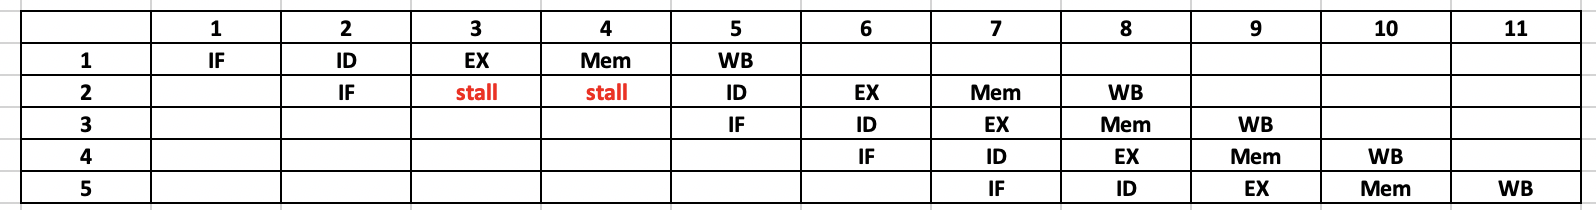
\includegraphics[width=1\textwidth]{q6p1}
\end{center}
بنابراین اجرای دستورات 
\textcolor{red}{11}
کلاک طول می کشد . با فرض این که پردازنده ۵ مرحله بوده با این توقف اجرای دستورات 
\textcolor{red}{6}
\lr{Clock Cycle}
بیشتر طول می کشد . 
\hrule
\section*{سوال ۷}
\subsection*{\textcolor{red}{الف}}
با توجه به این که معماری 
\lr{Single Cycle }
است بنابراین اجرای هر دستور یک کلاک طول می کشد بنابراین طول کلاک باید به اندازه ای باشد که طولانی ترین دستور نیز در یک کلاک انجام شود بنابراین برای این معماری دوره کلاک به صورت زیر است  :‌
\begin{center}
	\lr{Clock Cycle Time  = 400 ps  + 200 ps + 300 ps  + 500 ps  + 200 ps = 1600 ps}
\end{center}
\subsection*{\textcolor{red}{ب}}
با توجه به این که معماری 
\lr{Multi Cycle}
می باشد بنابراین به جای این که تمام مراحل اجرای یک دستور در یک کلاک انجام شود ، هر مرحله اجرا در یک کلاک انجام می شود بنابراین کلاک آن باید طوری باشد که طولانی ترین مرحله نیز به درستی انجام شود بنابراین دوره کلاک به صورت زیر است  : 
\begin{center}
	\lr{Clock Cycle Time  = MAX(400ps , 200ps , 300ps , 500ps  , 200ps) = 500 ps }
\end{center}
\hrule
\section*{سوال ۸}
\subsection*{\textcolor{red}{الف}}
با توجه به این که معماری 
\lr{Single Cycle }
می باشد بنابراین برای تمام دستورات 
\textcolor{red}{\lr{CPI = 1}}
پس برای انجام شدن تمام دستورات 
\lr{Load}
داریم  : 
\begin{center}
	\lr{\# of Clock Cycles = CPI * IC}\\
	\lr{IC = 1000000 * 0.25 = 250000}\\
	\lr{\# of Clock Cycles  = 1 * 250000 = 250000}
\end{center}
بنابراین برای انجام شدن تمام دستورات 
\lr{Load}
به 
\textcolor{red}{250000}
کلاک نیاز داریم  . 
\\
با توجه به معماری داریم  : 
\begin{center}
	\lr{Clock Cycle Time  = 400 ps + 200 ps + 300 ps + 500 ps + 200 ps  = 1600 ps}
\end{center}
بنابراین زمان اجرا برای این معماری به صورت زیر است  :‌
\begin{center}
	\lr{Execution Time  = IC * CPI * Clock Cycle Time = 250000 * 1 * 1600ps = 400000000 ps = 0.0004 s}
\end{center}
بنابراین برای اجرای تمام دستورات 
\lr{Load}
در این معماری نیاز به 
\textcolor{red}{0/0004}
ثانیه داریم  . 
\subsection*{\textcolor{red}{ب}}
با توجه به اسلاید های درس داریم  :
\begin{center}
	\lr{ALU  = 4 Clock Cycle}\\
	\lr{Load = 5 Clock Cycle}\\
	\lr{Store = 4 Clock Cycle}\\
	\lr{Branches = 3 Clock Cycle}
\end{center}
ابتدا مقدار 
\lr{CPI}
را به دست می آوریم ‌:
\begin{center}
	\lr{CPI = (4*0.5) + (3 * 0.15) + (5 * 0.25) + (4 * 0.1) = 4.1}
\end{center}
حال مانند حالت قبل برای تعداد کلاک های لازم برای اجرا شدن تمام دستورات 
\lr{Load}
داریم : 
\begin{center}
\lr{\# of Clock Cycles = IC * CPI = 250000 * 4.1  = 1025000 }
\end{center}
بنابرایت تعداد کلاک های لازم برابر است با 
\textcolor{red}{1025000}
\\
با توجه به معماری داریم  : 
\begin{center}
		\lr{Clock Cycle Time  = MAX(400ps , 200ps , 300ps , 500ps  , 200ps) = 500 ps }
\end{center}
و مانند حالت قبل برای زمان اجرا داریم  : 
\begin{center}
	\lr{Execution Time  = IC * CPI * Clock Cycle Time = 250000 * 4.1 * 500ps = 512500000 ps = 0.0005125}
\end{center}
بنابراین  اجرای تمام دستورات 
\lr{Load}
در این معماری 
\textcolor{red}{0/0005125}
ثانیه طول می کشد .  
\hrule
\section*{سوال ۹}
\begin{flushleft}
	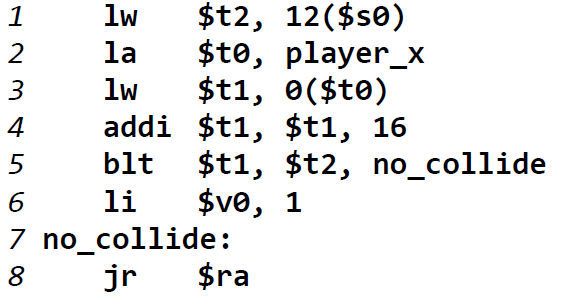
\includegraphics[width=0.5\textwidth]{q9p1}
\end{flushleft}
\subsection*{\textcolor{red}{الف}}
با توجه به بالا داریم  : 
\subsubsection*{1}
 خطوط 
\textcolor{red}{۱}
و
\textcolor{red}{۴}
با یک دیگر 
\textcolor{blue}{\lr{Structure Hazard}}
دارند . به این دلیل که در زمانی که دستور 
\lr{lw}
می خواهد مقداری را بخواند دستور 
\lr{addi}
می خواهد 
\lr{Fetch }
بشود که چون یک حافظه داریم این موضوع باعث به وجود آمدن 
\lr{Structure Hazard}
می شود  . 
\subsubsection*{2}
 خطوط 
\textcolor{red}{۳}
و 
\textcolor{red}{۶}
با یک دیگر 
\textcolor{blue}{\lr{Structure Hazard}}
دارند . مانند قبل در زمانی که دستور 
\lr{lw}
می خواهد از حافظه بخواند در همان زمان دستور 
\lr{li}
می خواهد 
\lr{Fetch}
شود که این به دلیل داشتن یک حافظه غیر ممکن است و باعث به وجود آمدن 
\lr{Structure Hazard}
می شود. 
\subsubsection*{3}
 خطوط
\textcolor{red}{2}
و 
\textcolor{red}{۳}
بر سر 
\lr{\$t0}
با یک دیگر 
\textcolor{blue}{\lr{Data Hazard}}
دارند . 
\subsubsection*{4}
خطوط 
\textcolor{red}{۳}
و 
\textcolor{red}{۴}
بر سر 
\lr{\$t1}
با یک دیگر 
\textcolor{blue}{\lr{Data Hazard}}
دارند. 
\subsubsection*{5}
خطوط 
\textcolor{red}{۴}
و
\textcolor{red}{۵}
بر سر 
\lr{\$t1}
با یک دیگر 
\textcolor{blue}{\lr{Data Hazard}}
دارند. 
\subsubsection*{6}
خطوط 
\textcolor{red}{۱} 
و 
\textcolor{red}{۵}
بر سر 
\lr{\$t2}
با یک دیگر 
\textcolor{blue}{\lr{Data Hazard}}
دارند . 
\\
این 
\lr{Hazrd}
ممکن است  به خاطر 
\lr{stall }
های موجود به وجود نیاید . ولی احتمال به وجود آمدنش صفر نیست  .
\subsubsection*{7}
بعد از دستور 
\lr{blt}
یک 
\textcolor{blue}{\lr{Control Hazard}}
به وجود می آید . 
\subsection*{\textcolor{red}{ب}}
در این حالت فقط باید برای مرحله 
\lr{MEM}
متوقف شویم که نمودار آن  به صورت زیر می باشد :‌

 
 \begin{center}
 	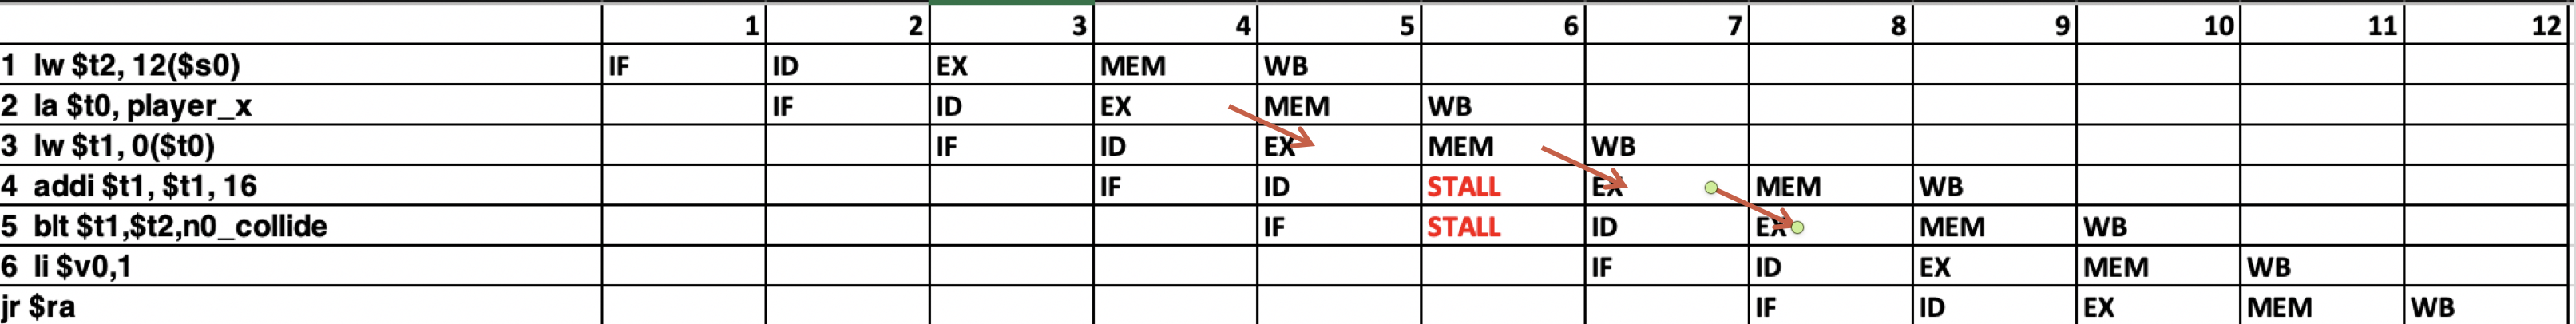
\includegraphics[width=1.1\textwidth]{q9p2a}
 \end{center}
بنابراین همان طور که می توان درنمودار دید در این حالت اجرای برنامه 
\textcolor{red}{12}
سیکل طول می کشد . 
\lr{Forward}
ها با فلش مشخص شده اند  . 

\end{document}